\chapter{Configuració de \textit{Grafana}}\label{ch:grafana-config}

Grafana és la nostra eina principal observabilitat, i que ens permetrà visualitzar els nostres casos d'ús.
Per poder fer-la servir l'haurem de configurar per tal que aquesta consumeixi de la nostra base de dades principal, InfluxDB.

\noindent \\
Malauradament, aquesta eina no incorpora suport directe amb MongoDB, per tant, l'anàlisi general sobre les metadades s'haurà de fer per separat. \\ \\

\section*{Connexió amb InfluxDB}\label{sec:influxdb-grafana-connection}

\noindent
Per afegir una font de dades a Grafana a les darreres versions es realitza a través de la pestanya \textit{Connections}.
Seguidament,  escollirem InfluxDB a l'apartat de ``Add new connections'', on podrem escollir diferents fonts de dades (\textit{data sources}). \\

\noindent
\begin{tcolorbox}[colback=blue!5!white, colframe=blue!75!black, title=Llenguatge de cerca]
    InfluxDB suporta diferents llenguatges per realitzar les seves consultes.
    Però, el recomanable i més actualitzat és \textit{Flux}.
    Això és important pel fet que la configuració varia en funció del llenguatge escollit.
\end{tcolorbox}

\noindent \\
Escollirem el llenguatge Flux.
Les altres opcions són \textit{InfluxQL} i \textit{SQL}, no les farem servir.
Ara passem a la configuració.

\clearpage

\noindent
Per l'apartat d'HTTP (figura~\ref{fig:grafana-influxdb-http}) definirem l'\gls{URL} del servei.
Com el servei \gls{DNS} de la xarxa de \gls{Docker} ja resol el servei pel seu nom, l'hem de definir per \textbf{influxdb}.
Utilitzar \textbf{localhost} podria errar durant l'intent de connexió.

\begin{figure}[htbp]
    \centerline{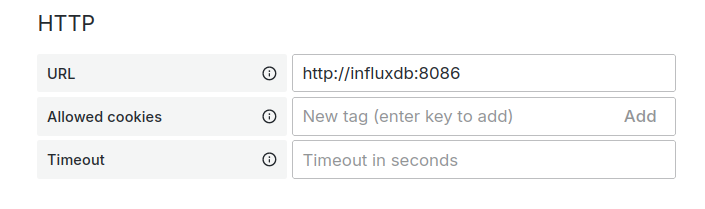
\includegraphics[width=\textwidth]{figures/grafana-influxdb-http}}
    \captionsetup{justification=centering}
    \caption[Configuració HTTP d'InfluxDB a \textit{Grafana}.]{Configuració HTTP d'InfluxDB a \textit{Grafana}. (\textbf{Font}: Aplicatiu \textit{Grafana} del servidor de treball.)}\label{fig:grafana-influxdb-http}
\end{figure}

\noindent \\
Pel que fa a l'autenticació (figura~\ref{fig:grafana-influxdb-auth}), afegirem les nostres credencials d'\textbf{InfluxDB}.
La paraula clau \textbf{configured} indica que la contrasenya ja ha sigut introduïda, i no que aquesta sigui ``configured''.

\begin{figure}[htbp]
    \centerline{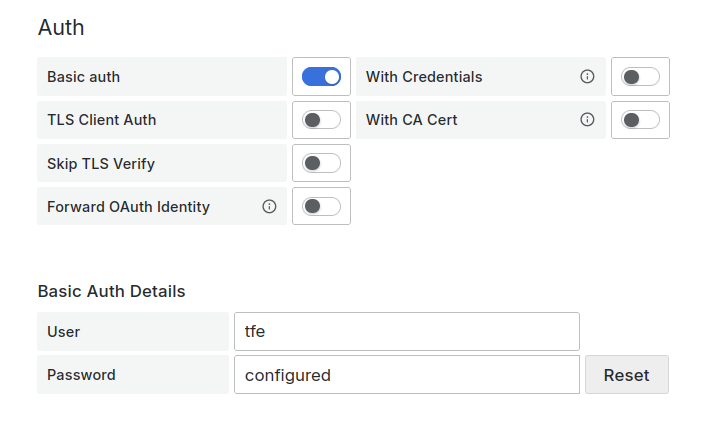
\includegraphics[width=0.9\textwidth]{figures/grafana-influxdb-auth}}
    \captionsetup{justification=centering}
    \caption[Configuració d'autenticació d'InfluxDB a \textit{Grafana}.]{Configuració d'autenticació d'InfluxDB a \textit{Grafana}. (\textbf{Font}: Aplicatiu \textit{Grafana} del servidor de treball.)}\label{fig:grafana-influxdb-auth}
\end{figure}

\clearpage
\noindent
Finalment, completarem els detalls d'InfluxDB (figura~\ref{fig:grafana-influxdb-details}), que són l'organització i els altres paràmetres definits durant la configuració d'InfluxDB.
El \textit{token} és el clau que utilitzarem com autenticació a l'hora de realització de consultes.

\noindent \\
Aquest \textit{token} es genera a la interfície de la base de dades.
Hem de tenir en compte d'assignar els permisos de lectura/escriptura correctes.
D'altra manera, no podrem realitzar les consultes pertinents.

\begin{figure}[htbp]
    \centerline{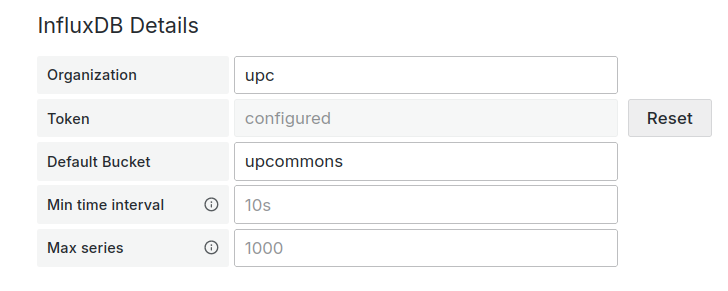
\includegraphics[width=\textwidth]{figures/grafana-influxdb-details}}
    \captionsetup{justification=centering}
    \caption[Configuració dels detalls d'InfluxDB a \textit{Grafana}.]{Configuració dels detalls d'InfluxDB a \textit{Grafana}. (\textbf{Font}: Aplicatiu \textit{Grafana} del servidor de treball.)}\label{fig:grafana-influxdb-details}
\end{figure}

\clearpage

\section*{Creació de \textit{dashboards}}\label{sec:grafana-dashboards}

\noindent
Afegir panells de visualització és una tasca senzilla un cop tens definit el teu cas d'ús, les dades que vols tractar i quin tipus de representació visual vols realitzar.

\noindent \\
Els passos són:
\begin{center}
    Dashboards \(\rightarrow\) New Dashboard \(\rightarrow\) Add Visualization
\end{center}

\noindent
Has d'escollir la font de dades.
Apareixerà l'InfluxDB que prèviament s'ha configurat.
Seguidament emergeixen tres finestres principals, adaptables en mida.

\noindent \\
La finestra central de la figura~\ref{fig:grafana-main-panel} mostrarà la representació de les dades.
La finestra central de la figura~\ref{fig:grafana-main-panel} mostrarà la representació de les dades.
A la part inferior, hi ha un editor on es pot introduir la cerca a InfluxDB.
Un cop introduïda, s'emmagatzema i s'executa automàticament.

\begin{figure}[htbp]
    \centerline{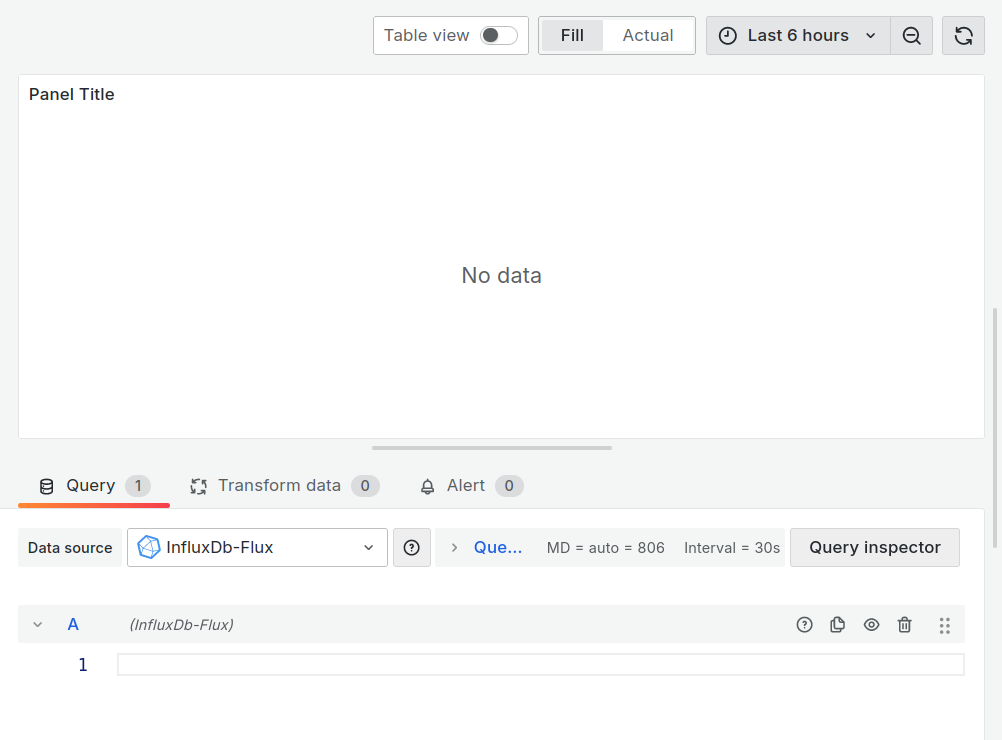
\includegraphics[width=\textwidth]{figures/grafana-main-panel}}
    \captionsetup{justification=centering}
    \caption[Finestra principal d'un panell de \textit{Grafana}.]{Finestra principal d'un panell de \textit{Grafana}. (\textbf{Font}: Aplicatiu \textit{Grafana} del servidor de treball.)}\label{fig:grafana-main-panel}
\end{figure}

\clearpage

\noindent
A la part dreta (figura~\ref{fig:grafana-panel-visualization}) es troba una finestra per personalitzar el panell, tant colors, llegenda, estils, etcètera.
L'opció més important es troba a la part superior, on pots definir el tipus de representació: sèrie temporal, diagrama de barres, intensitat de colors, histogrames, i infinites més opcions.
Sempre que s'adaptin les dades per cada tipus de representació, endavant!

\begin{figure}[h]
    \centering
    \begin{subfigure}{0.45\textwidth}
        \centering
        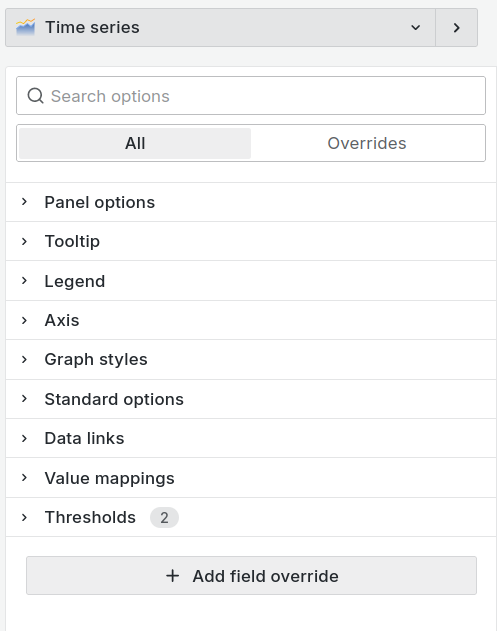
\includegraphics[width=\linewidth]{figures/grafana-panel-customization}
        \label{fig:figure1}
    \end{subfigure}
    \hspace{0.05\textwidth}
    \begin{subfigure}{0.45\textwidth}
        \centering
        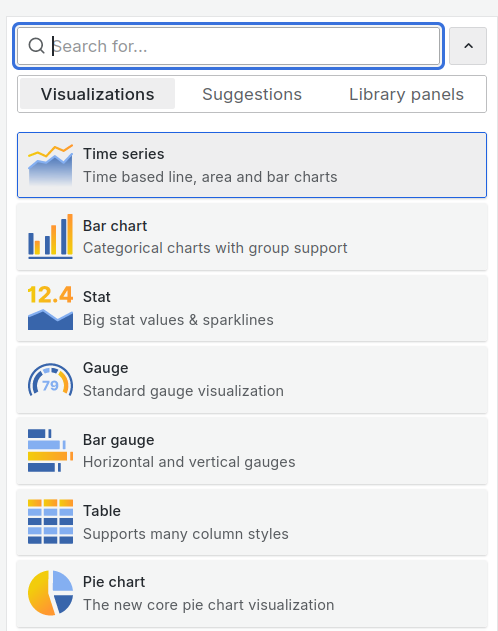
\includegraphics[width=\linewidth]{figures/grafana-panel-visualization-type}
        \label{fig:figure2}
    \end{subfigure}
    \captionsetup{justification=centering}
    \caption[Esquerra: Personalització dels panells de \textit{Grafana}. Dreta: Tipus de visualització pels panells de \textit{Grafana}.]{Esquerra: Personalització dels panells de \textit{Grafana}. \\ Dreta: Tipus de visualització pels panells de \textit{Grafana}. (\textbf{Font}: Aplicatiu \textit{Grafana} del servidor de treball.)}
    \label{fig:grafana-panel-visualization}
\end{figure}
